\documentclass{report}
\usepackage{geometry}
 \geometry{
 a4paper,
 total={170mm,257mm},
 left=20mm,
 top=20mm,
 }
\usepackage[latin1]{inputenc}% erm\"oglich die direkte Eingabe der Umlaute 
\usepackage[T1]{fontenc} % das Trennen der Umlaute
\usepackage{ngerman} % hiermit werden deutsche Bezeichnungen genutzt und 
                     % die W\"orter werden anhand der neue Rechtschreibung 
             % automatisch getrennt. 
\usepackage{graphicx}
\usepackage{comment}
\usepackage{hyperref}
\graphicspath{ {./} }
\usepackage{subcaption}
\newcommand{\sectionbreak}{\clearpage}
\usepackage[section]{placeins}
\title{Short Documentation of SRC analysis}
\begin{document}

\maketitle

\section{Setup}
Beam energy: 400 AMeV\newline
Beamtype: 12C\newline
Target: CH2\newline
Beam Time: 3 hours\newline
Tracking detectors: MWPC 1,2,3 (just x position)\newline
ToF measurement: START to ToFW\newline
Charge Measurement: TWIM Music\newline
Event selection criteria for CALIFA: two hits with E\textunderscore hit $> 30$ MeV (laboratory system) and 10B(11B) as daughter particle (exclusive events).\newline
No other cuts (for now).\newline

\section{12C(p,2p)11B analysis}
The Energy and momentum conservation for this reaction can be expressed as:\newline
$\bar{p}_{12C} + \bar{p}_{tg} = \bar{p}_{1} + \bar{p}_{2} + \bar{p}_{11B}$ (four momentum vectors) \newline
Assuming QE scattering in the mean field we approximate:\newline
$\bar{p}_{12C} = \bar{p}_{i} + \bar{p}_{11B}$ where $\bar{p}_{i}$ is the initial proton-four-momentum inside the 12C ion.\newline
Hence we obtain:\newline
$\bar{p}_{i} \approx \bar{p}_{miss} \equiv \bar{p}_{1} + \bar{p}_{2} - \bar{p}_{tg}$ \newline
And the missing Energy $E_{miss}$ is defined as:\newline
$E_{miss} \equiv m_{p} - e_{miss}$ (where $e_{miss}$ is the energy component of $\bar{p}_{miss}$ in the 12C frame).\newline
\subsection{Plots:}
The analysis of the missing momentum (components) is summarized in following plots:\newline
\begin{figure}[!htb]
  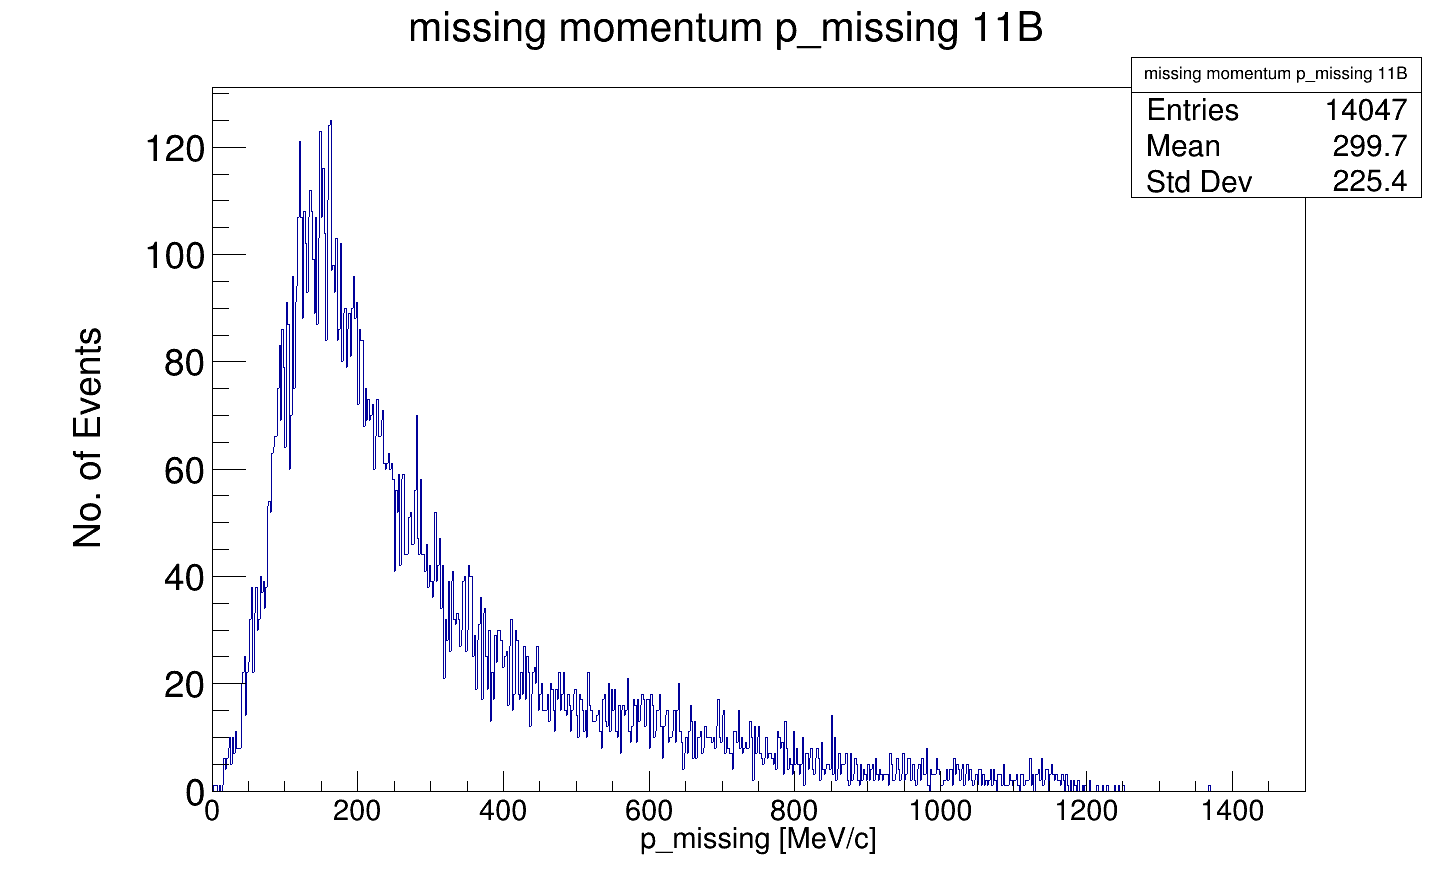
\includegraphics[width=\linewidth]{missing_mom_11B.png}
  \caption{Momentum of the initial proton inside the 12C ion.}
\end{figure}
\begin{figure}[!htb]
  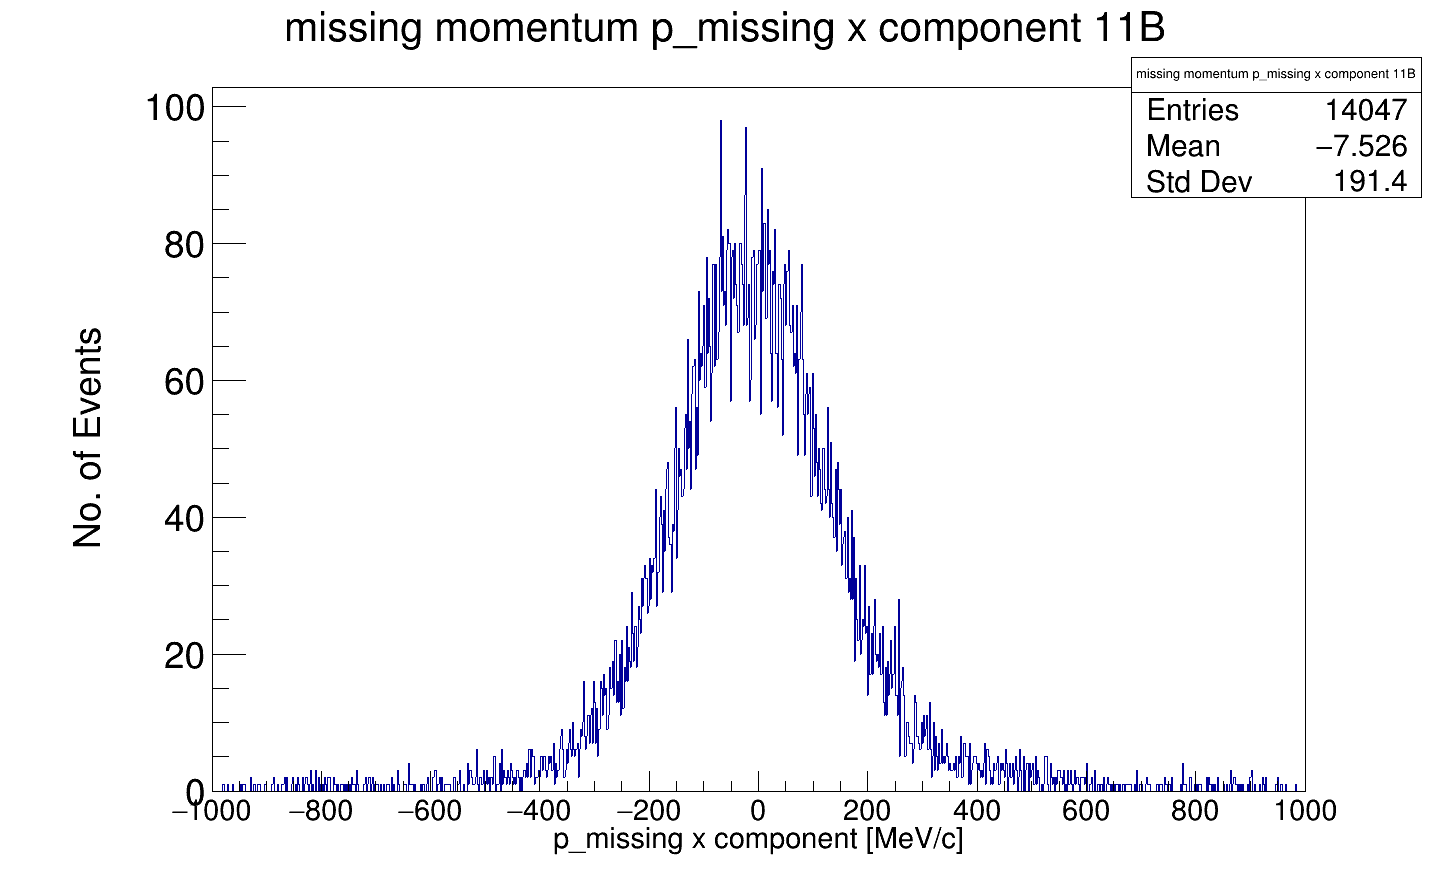
\includegraphics[width=\linewidth]{missing_mom_11B_x_comp.png}
  \caption{Momentum of the initial proton inside the 12C ion - x component.}
\end{figure}
\begin{figure}[!htb]
  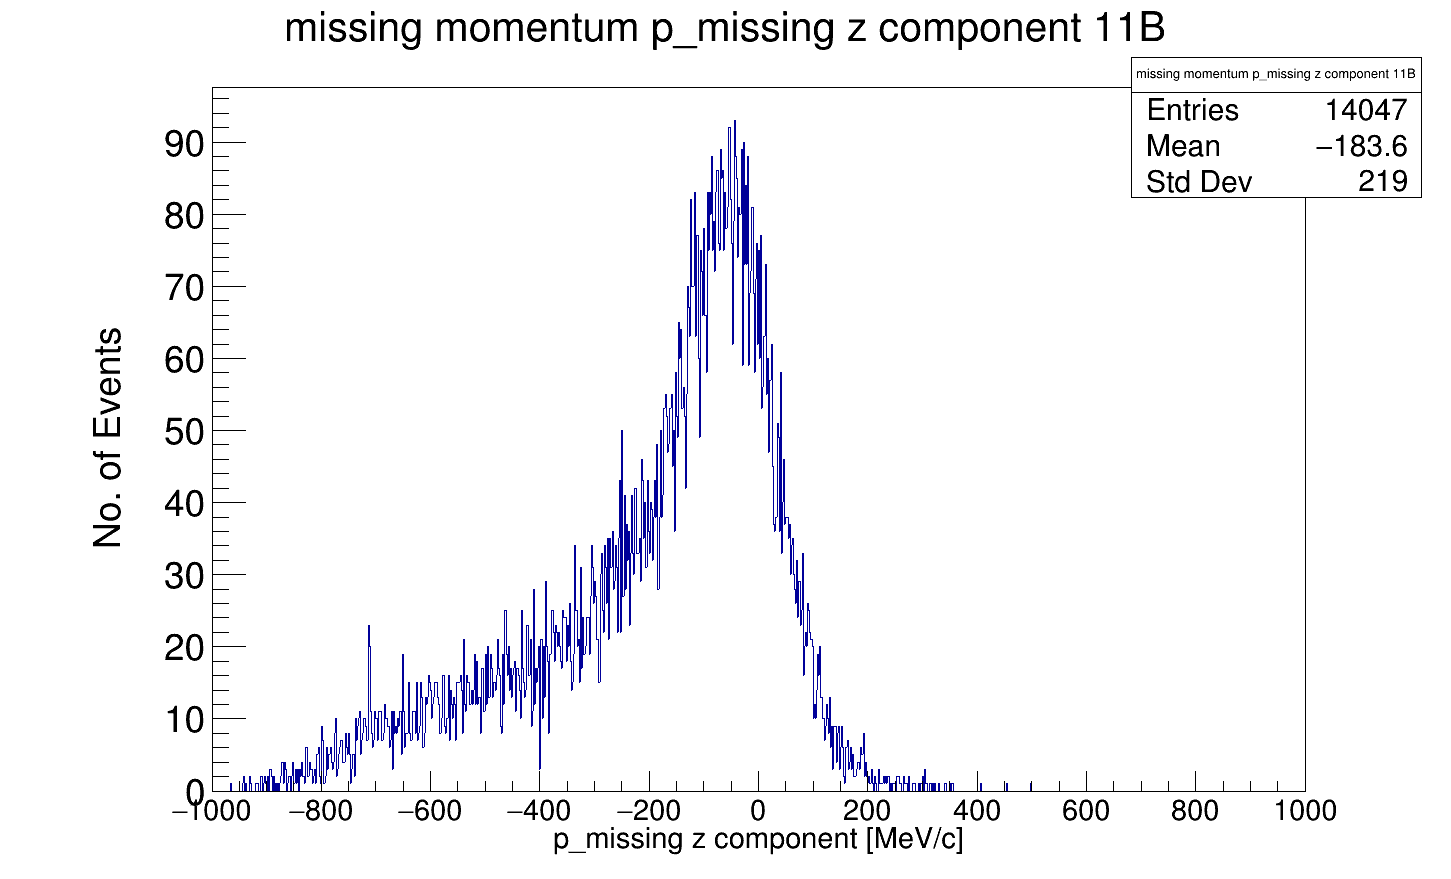
\includegraphics[width=\linewidth]{missing_mom_11B_z_comp.png}
  \caption{Momentum of the initial proton inside the 12C ion - z component. The shift in $p_{miss_z}$ is associated with a strong pp cross-section scaling with c.m. energy.}
\end{figure}
\newpage
The plots relating to the missing energy $E_{miss}$ are summarized in the following plots:\newline
\begin{figure}[!htb]
  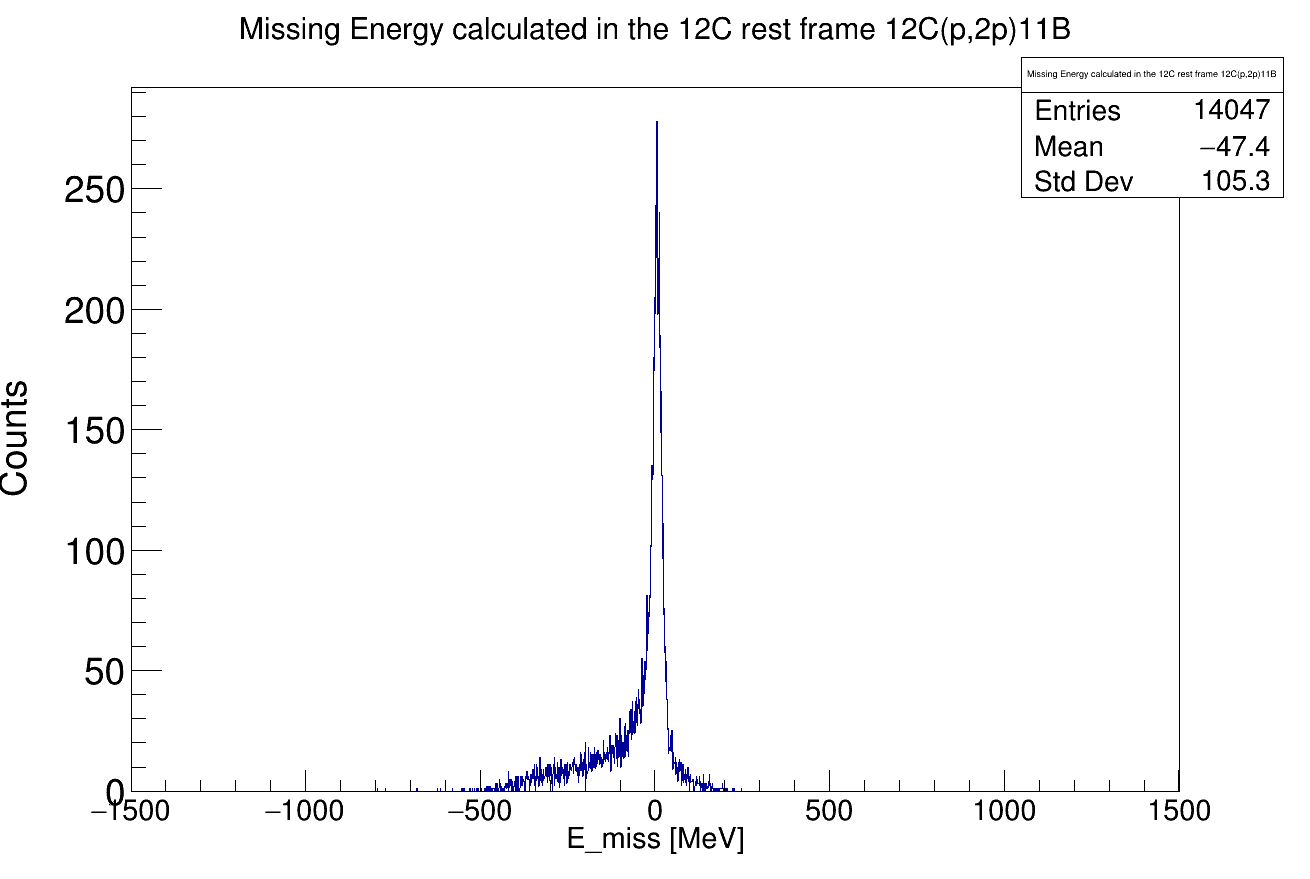
\includegraphics[width=\linewidth]{missing_E_12C_11B.png}
  \caption{Missing energy calculated in teh 12C rest frame.}
\end{figure}
\begin{figure}[!htb]
  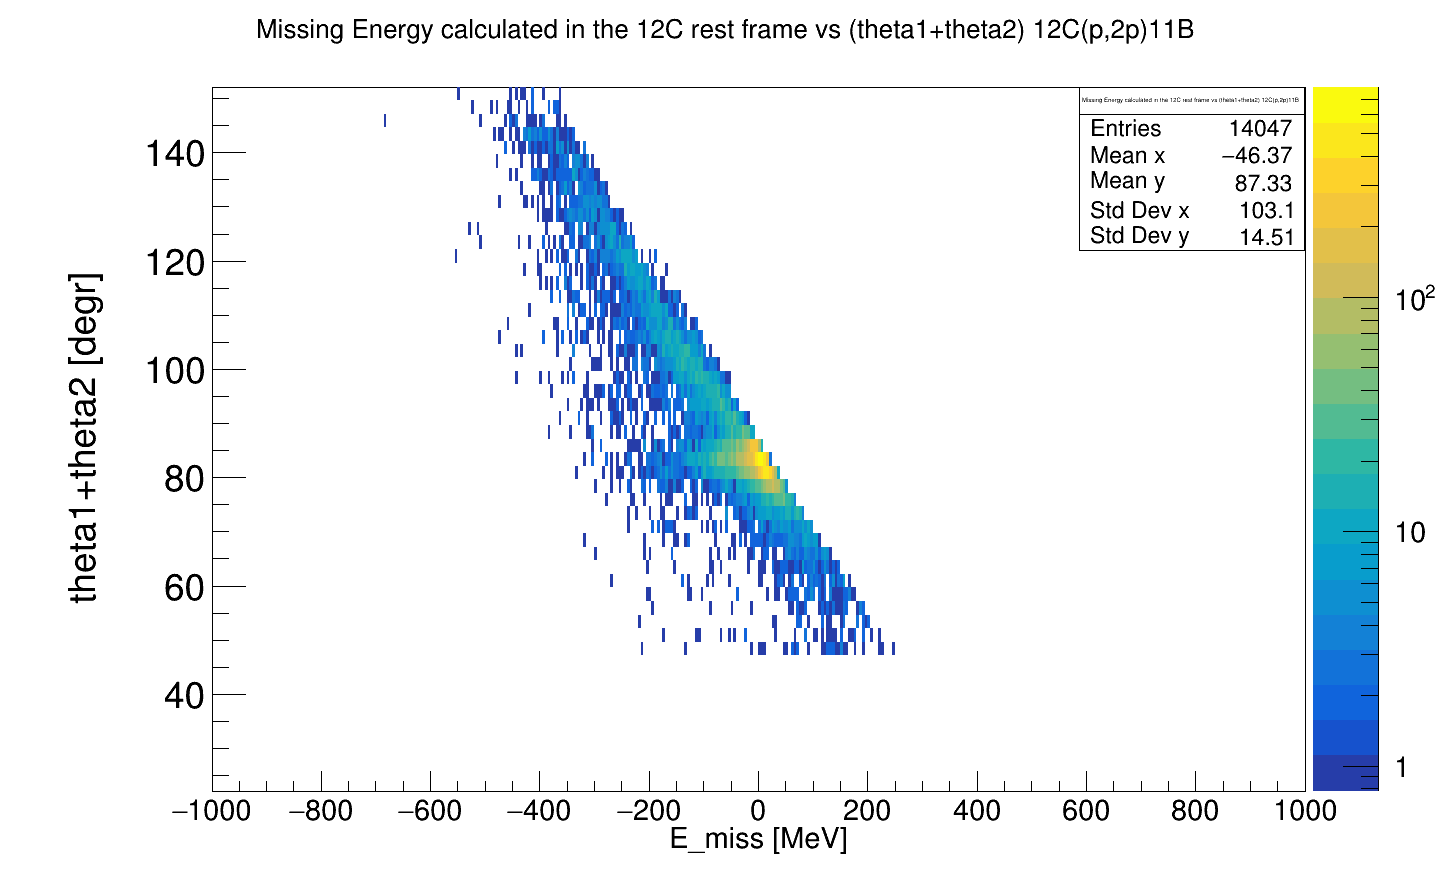
\includegraphics[width=\linewidth]{missing_E_12C_11B_vs_theta.png}
  \caption{Missing energy calculated in teh 12C rest frame versus theta1 + theta2. Most of the reactions are in the QE scattering region.}
\end{figure}
\newline
\newpage

The plots relating to the angular distribution of the two protons from the 12C(p,2p)11B reaction:\newline
\begin{figure}[!htb]
  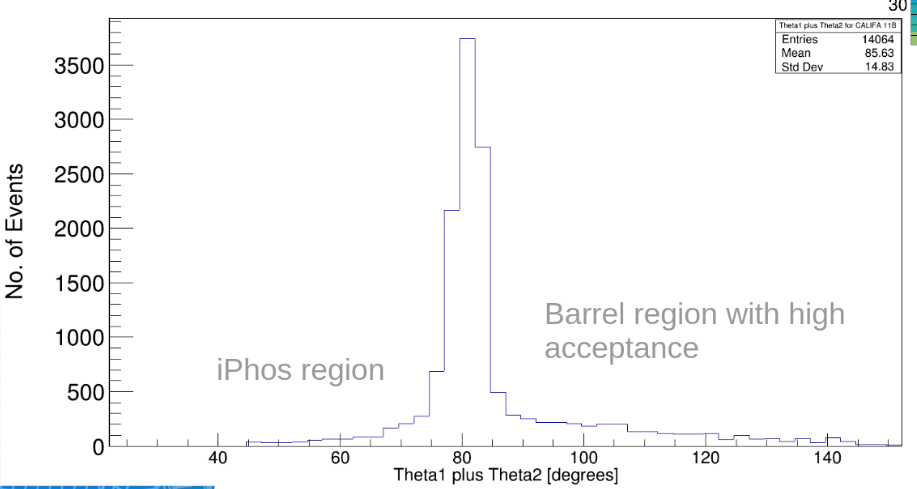
\includegraphics[width=\linewidth]{theta1_plus_theta2.png}
  \caption{Theta1 plus theta2 for proton 1 and proton 2 distribution.}
\end{figure}
\begin{figure}[!htb]
  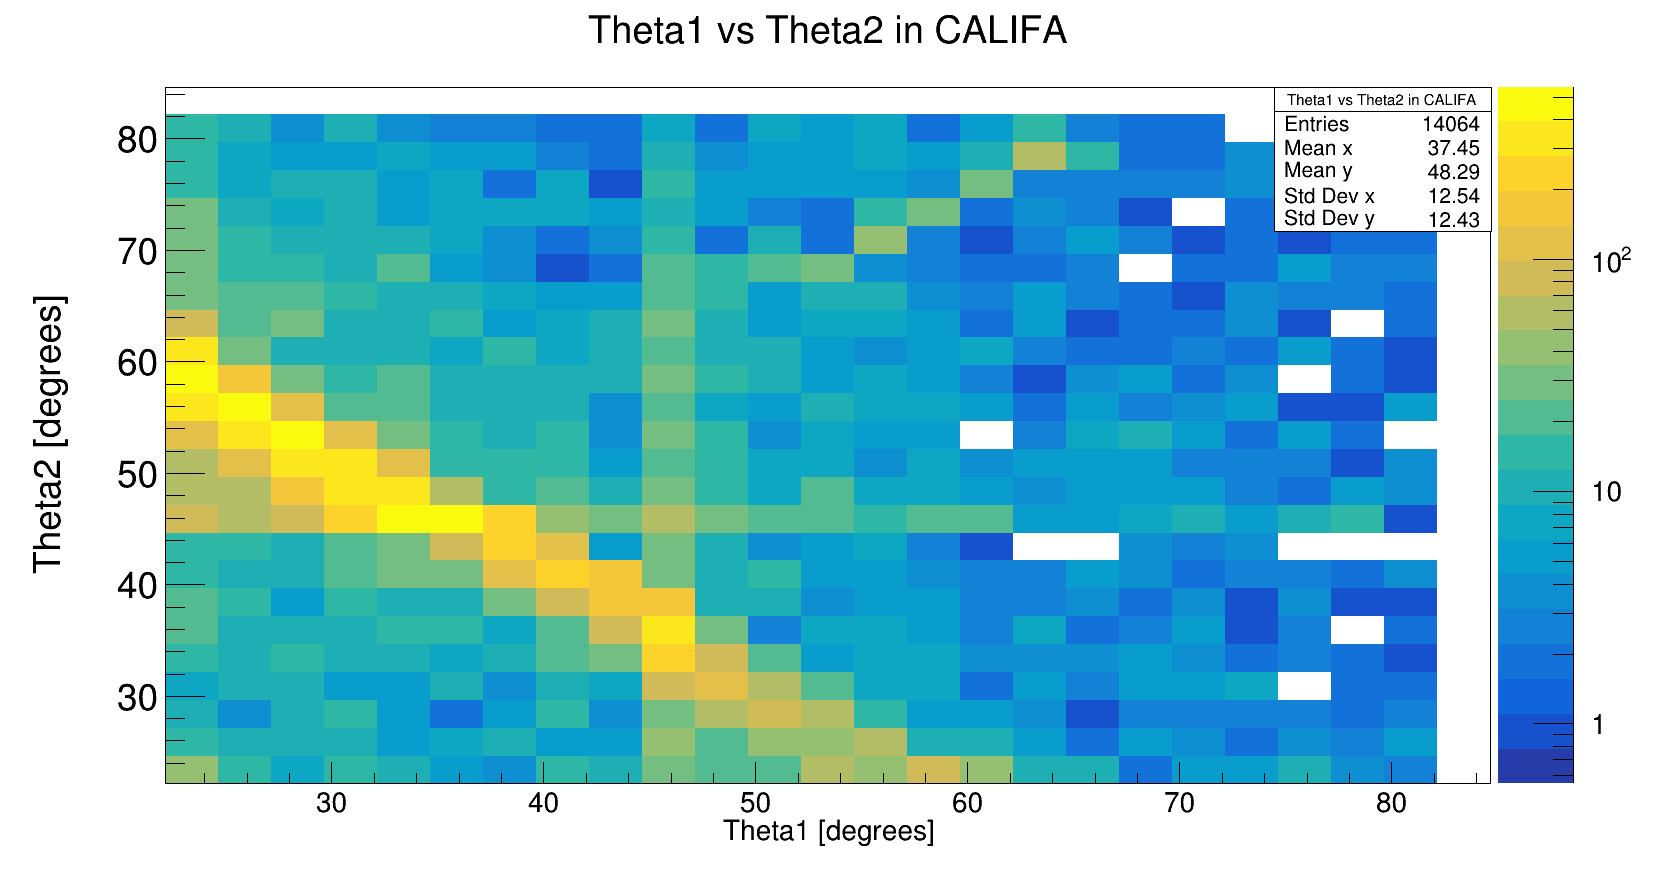
\includegraphics[width=\linewidth]{theta1_vs_theta2_right_binning.png}
  \caption{Theta1 vs theta2 for proton 1 and proton 2 where proton 1 is the one with higher kinetic energy.}
\end{figure}
\begin{figure}[!htb]
  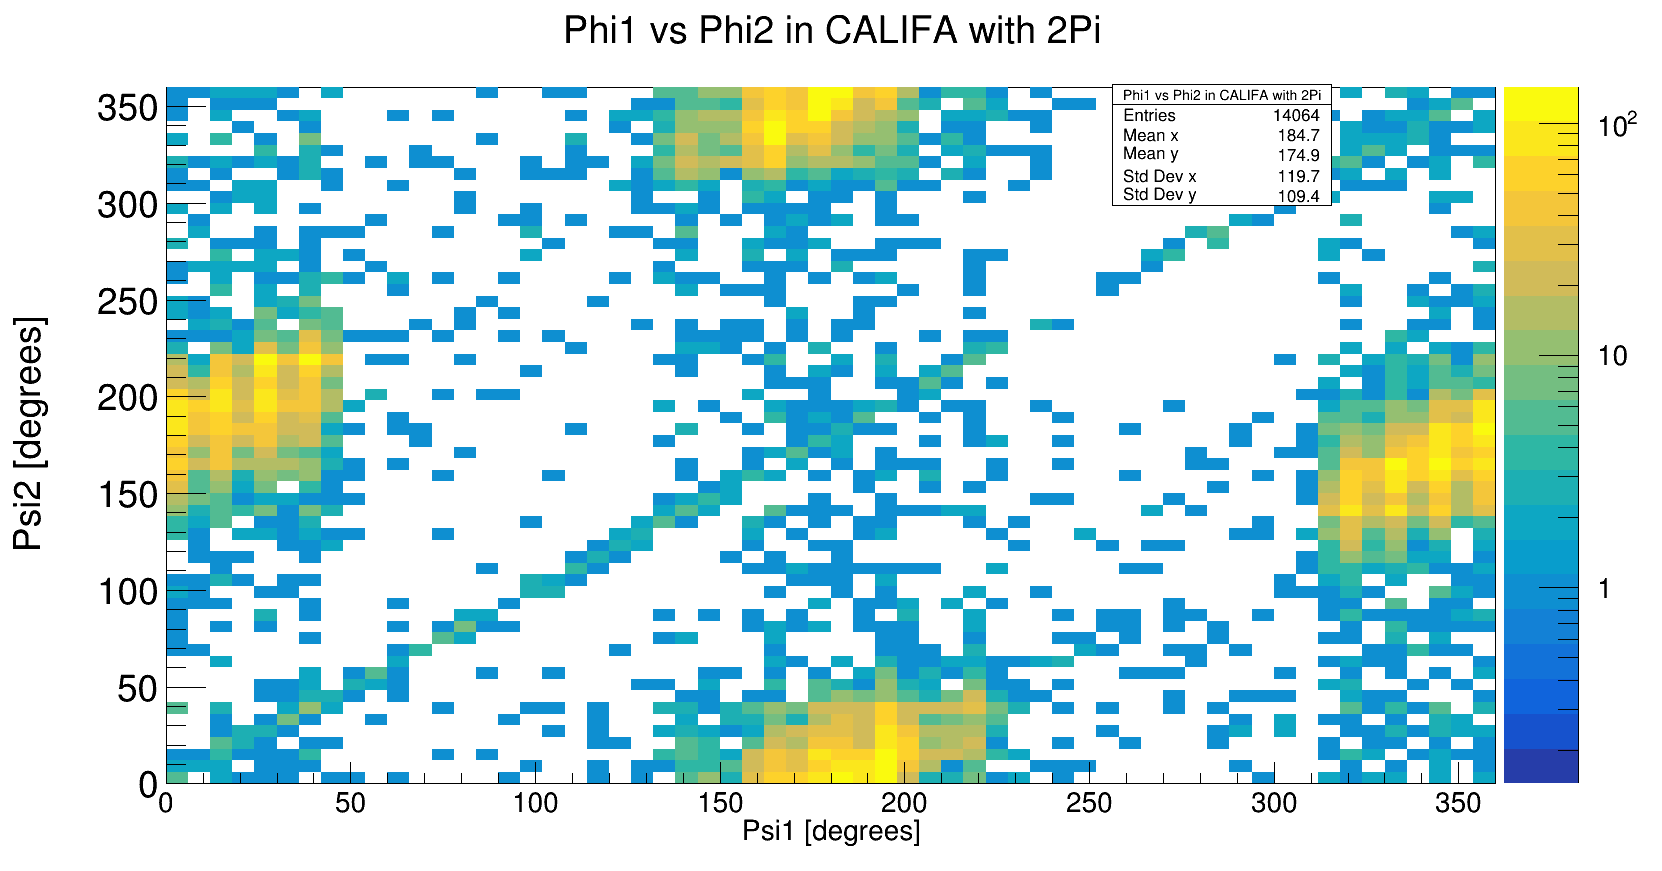
\includegraphics[width=\linewidth]{psi1_vs_psi2.png}
  \caption{Arzimuthal angular distribution for proton 1 and proton 2.}
\end{figure}
\newline
\begin{figure}[!htb]
  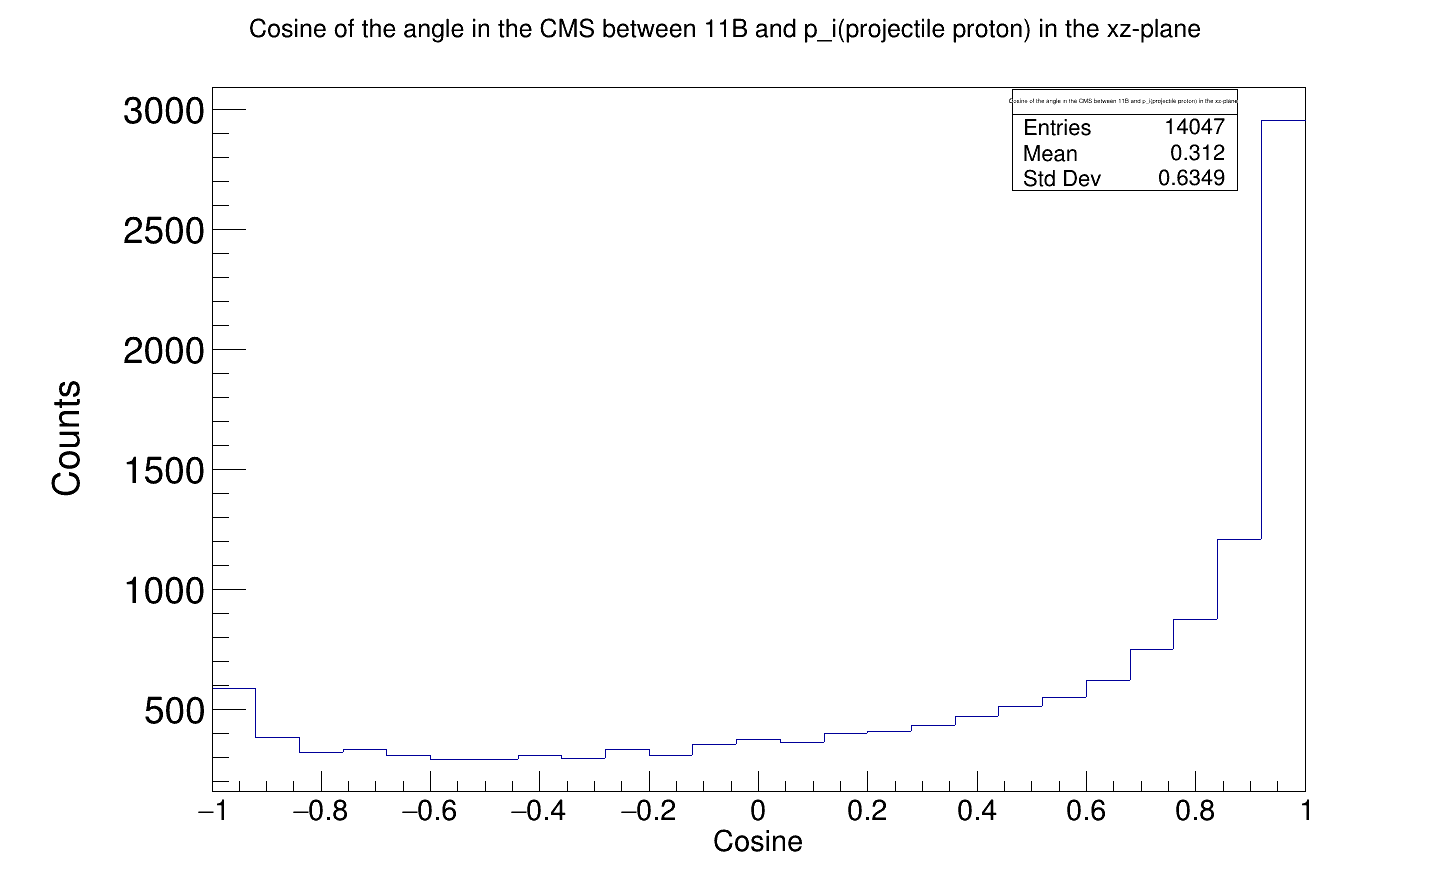
\includegraphics[width=\linewidth]{cos_11B_p_i.png}
  \caption{Cosine of the opening angle between the missing and fragment moment in 12C c.m. frame.}
  \label{fig:11b_p_i_distr}
\end{figure}
\newline
\newpage

As gamma spectrum related to the 12C(p,2p)11B reaction we get:\newline
\begin{figure}[!htb]
  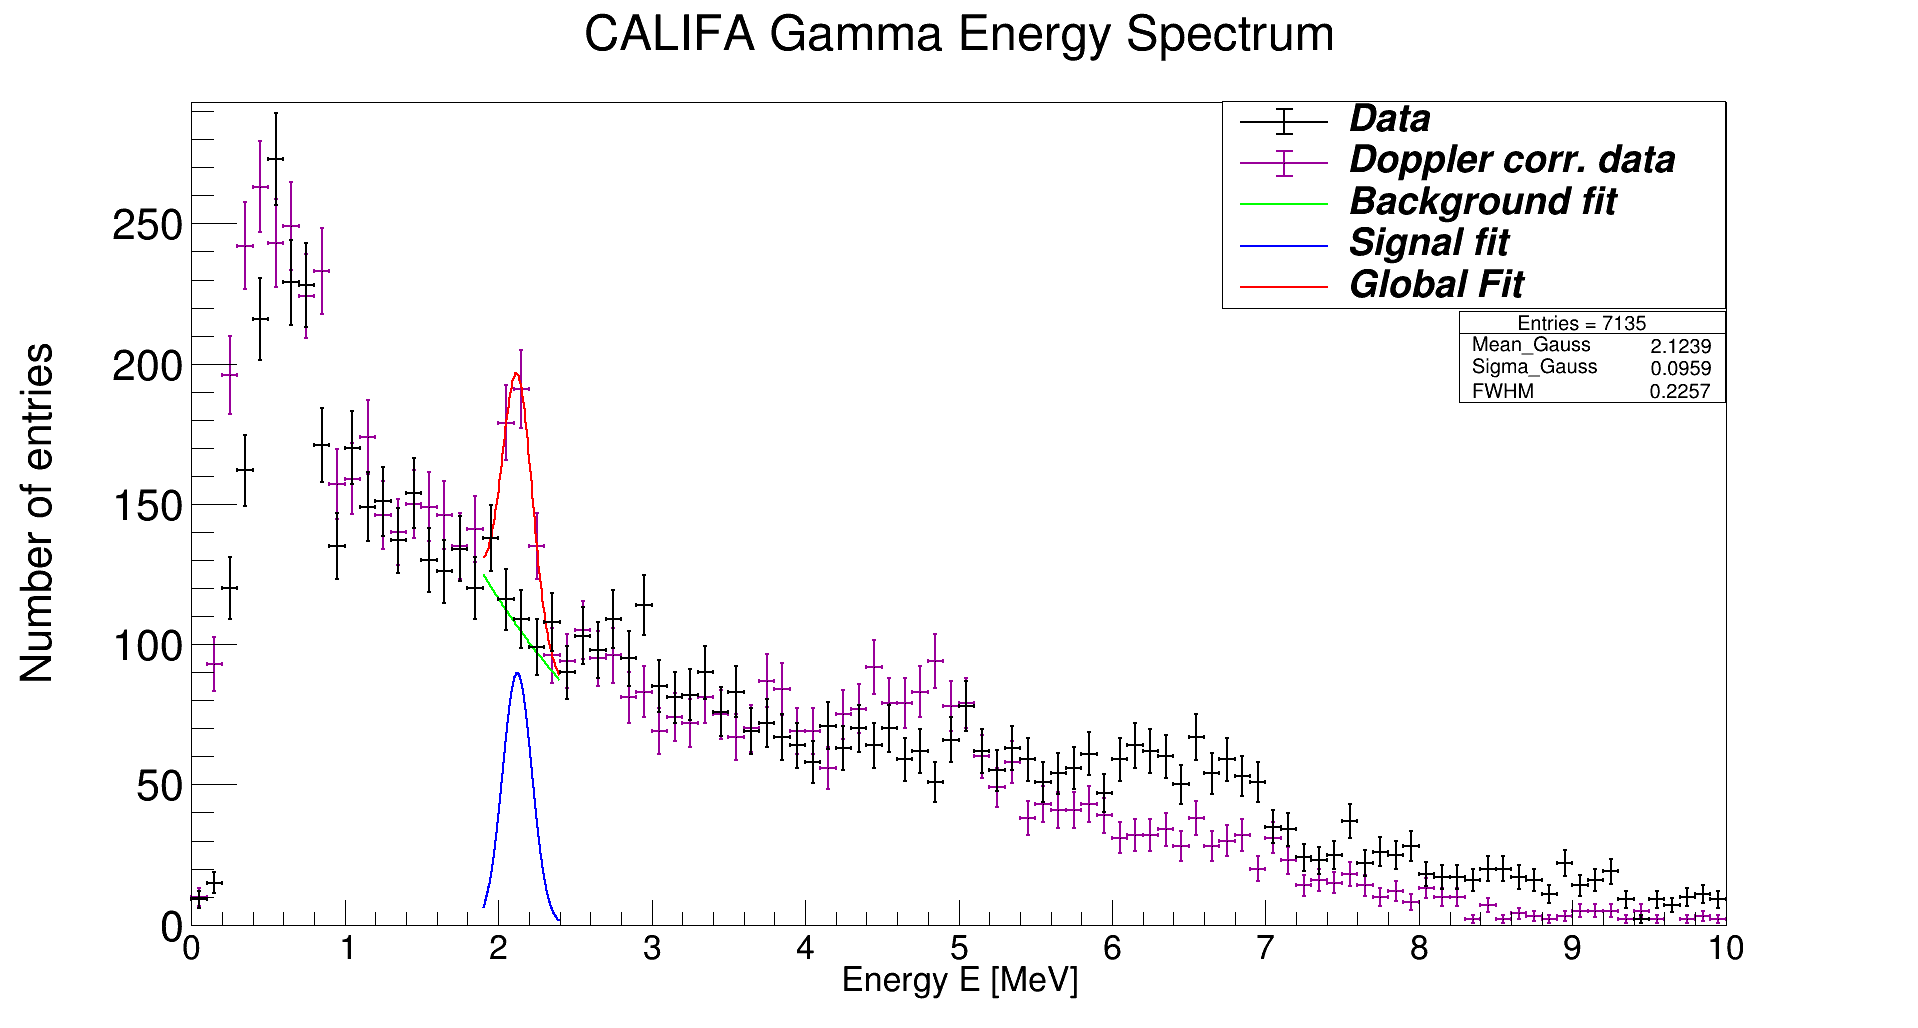
\includegraphics[width=\linewidth]{gamma_spec.png}
  \caption{Doppler reconstructed gamma spectrum for the first excited states (with a resolution around $10\%$).}
\end{figure}
\newline

\section{12C(p,2p)10B}
For this reaction the missing momentum (which equals to the initial proton momentum inside the 12C ion) is same as before:\newline
$\bar{p}_{i} \approx \bar{p}_{miss} \equiv \bar{p}_{1} + \bar{p}_{2} - \bar{p}_{tg}$ \newline
The missing nucleon mass in the entire reaction is given by:\newline
$M^2_{miss,excl} = \big(\bar{p}_{12C} + \bar{p}_{tg} - \bar{p}_{1} - \bar{p}_{2} - \bar{p}_{10B}\big)^2$\newline
The analysis of the missing momentum is summarized in following plots:\newline
\begin{figure}[!htb]
  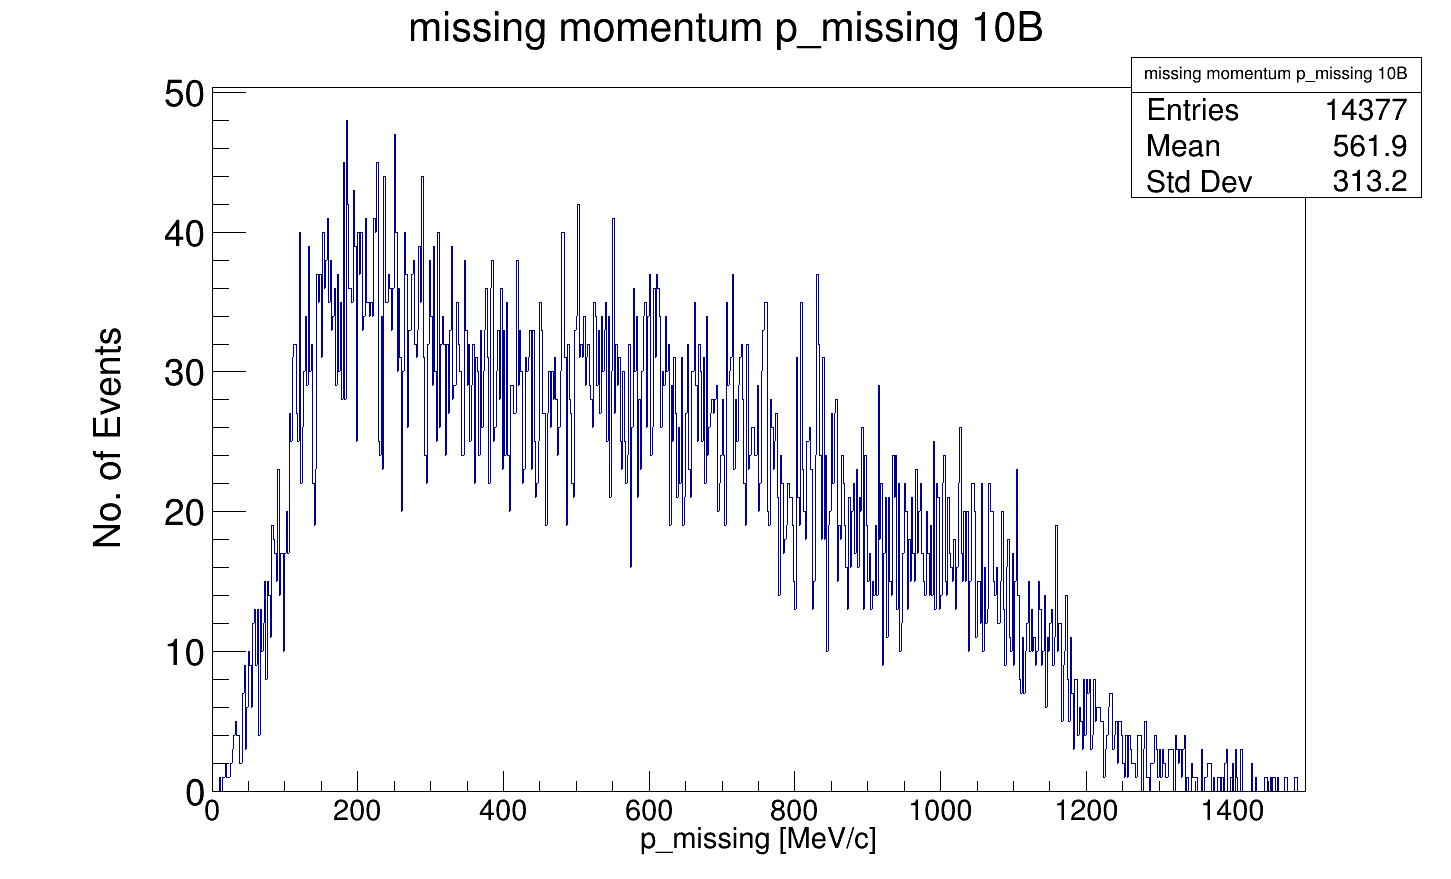
\includegraphics[width=\linewidth]{missing_mom_12C_10B.png}
  \caption{Initial proton momentum inside the 12C ion for the 12C(p,2p)10B reaction.}
\end{figure}
\newline
\begin{figure}[!htb]
  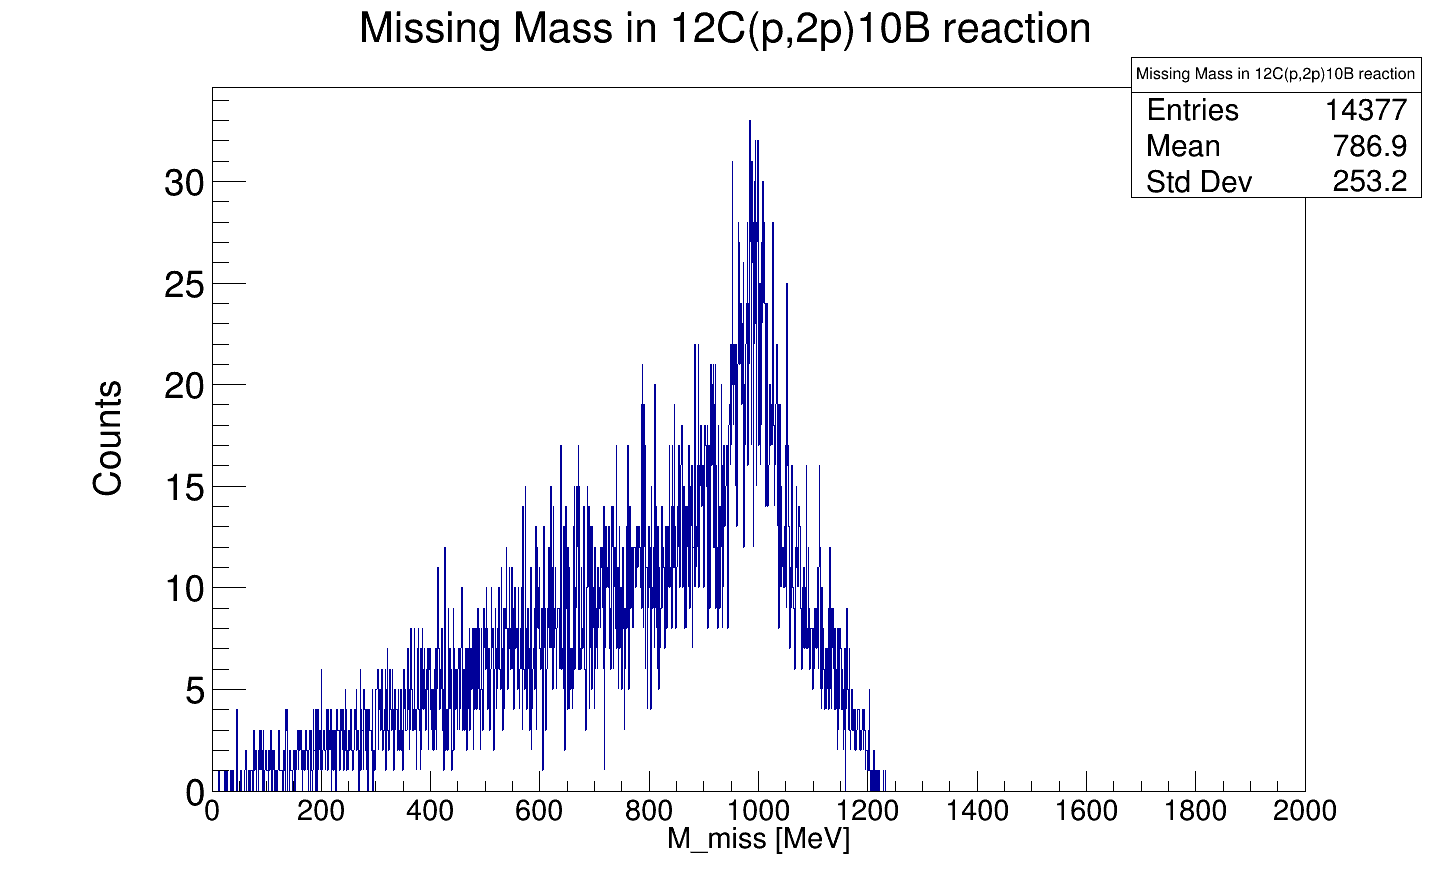
\includegraphics[width=\linewidth]{missing_mass_12C_10B.png}
  \caption{Missing mass with a peak $\approx m_{N}$ (where $m_{N}$ is the nucleon mass).}
\end{figure}
\newline
\newpage

To compare the missing momentum between the 12C(p,2p)11B and 12C(p,2p)10B reaction:\newline
\begin{figure}[!htb]
  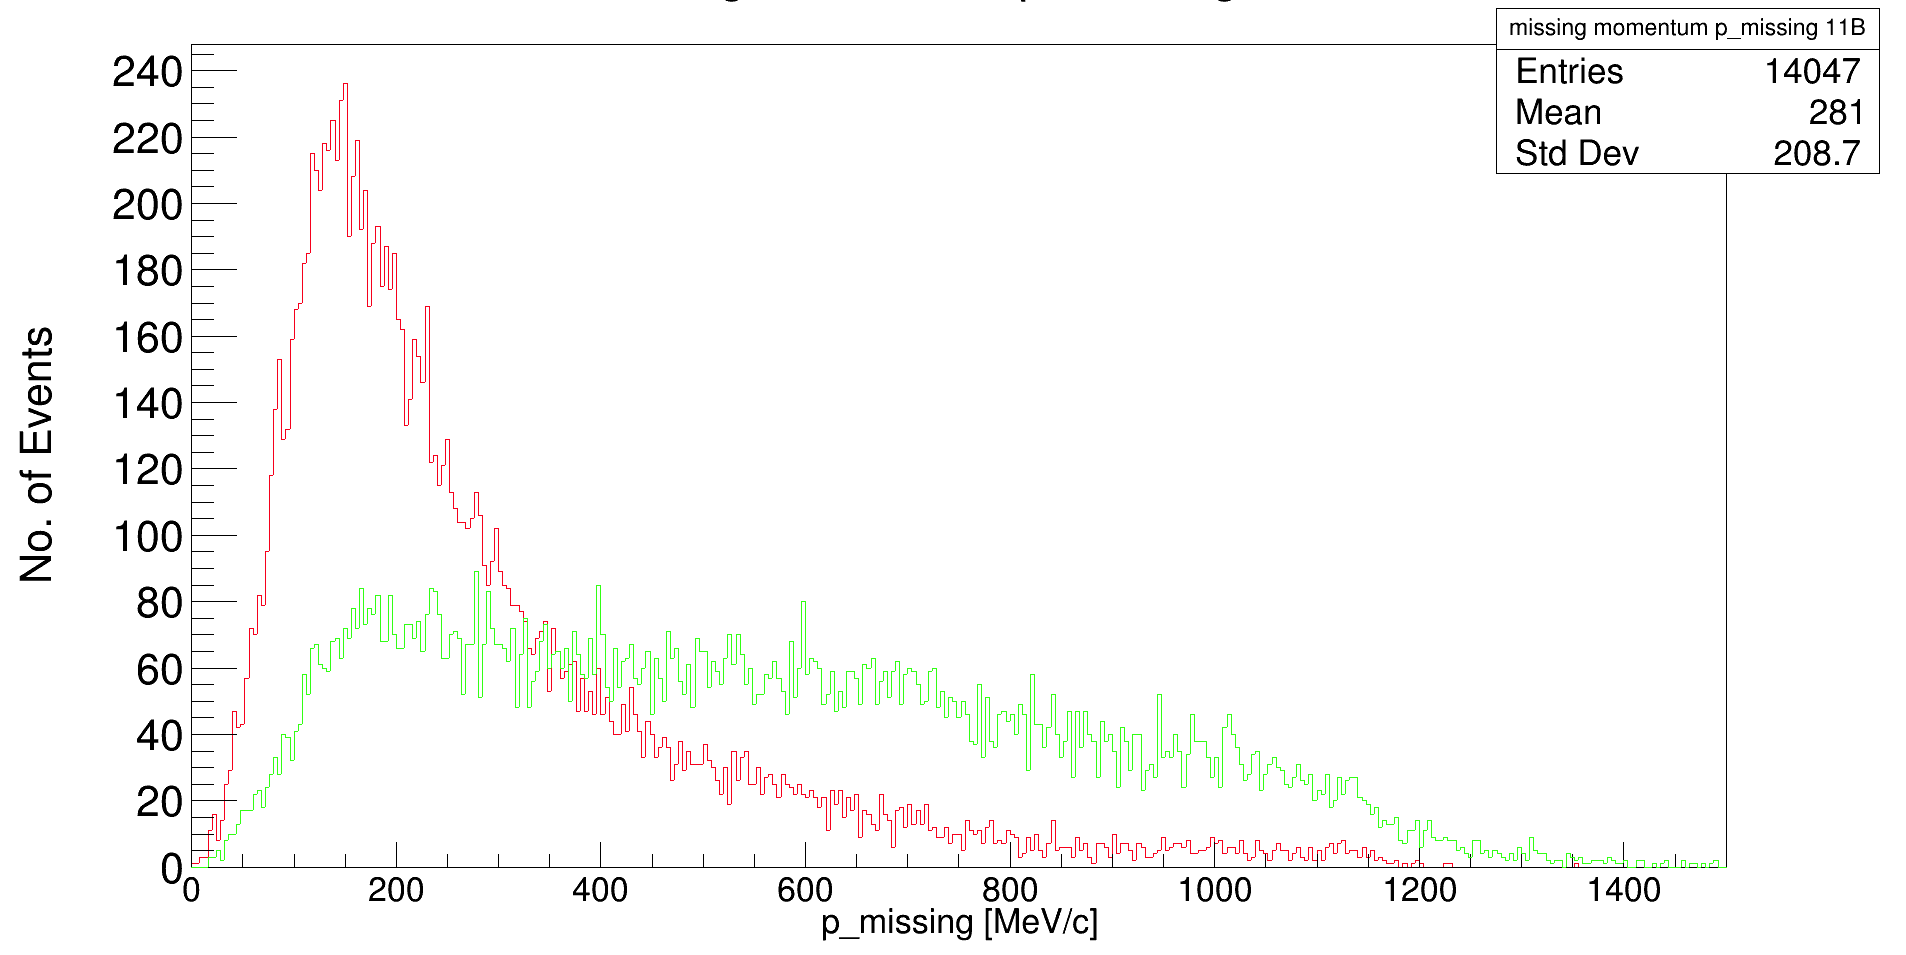
\includegraphics[width=\linewidth]{missing_mom_compare.png}
  \caption{Red: missing momentum for 12C(p,2p)11B reaction. Green: missing momentum for 12C(p,2p)10B reaction.}
\end{figure}
\newline
\newpage

The plots relating the angular distributions:\newline
\begin{figure}[!htb]
  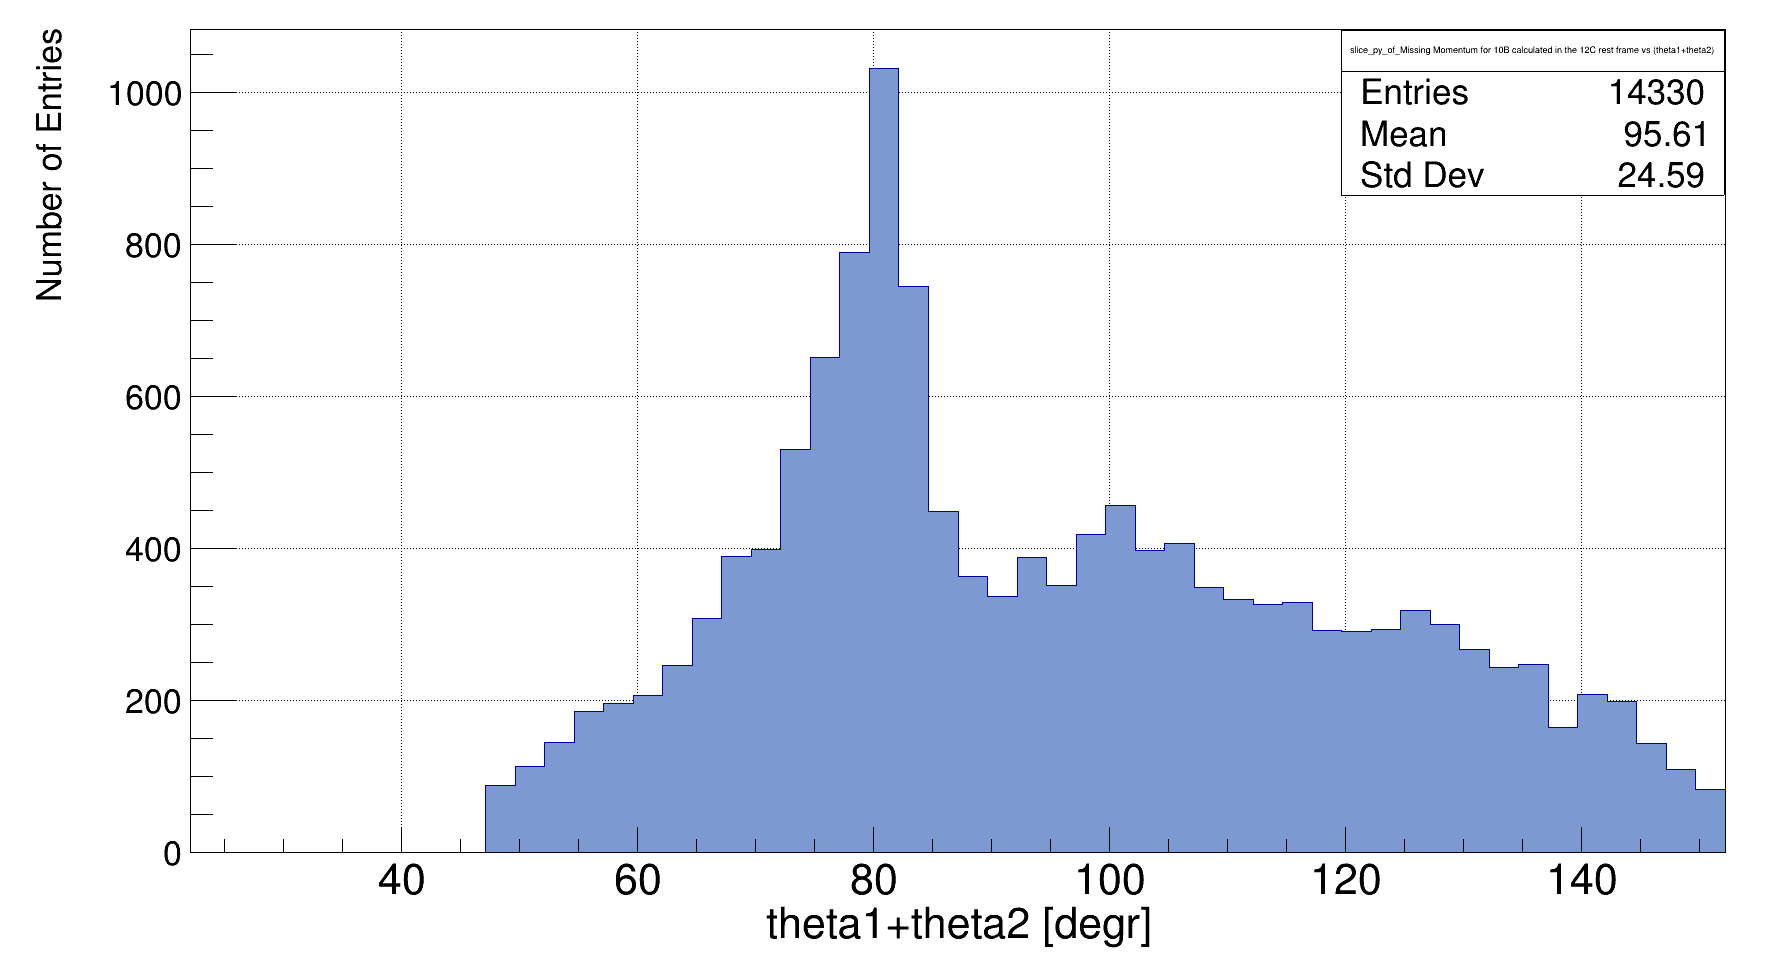
\includegraphics[width=\linewidth]{theta1_plus_theta2_src.png}
  \caption{Theta1 plus theta2 for the outgoing protons (or proton and deuteron??).}
  \label{fig:theta1_theta2_distr}
\end{figure}
\newline
\begin{figure}[!htb]
  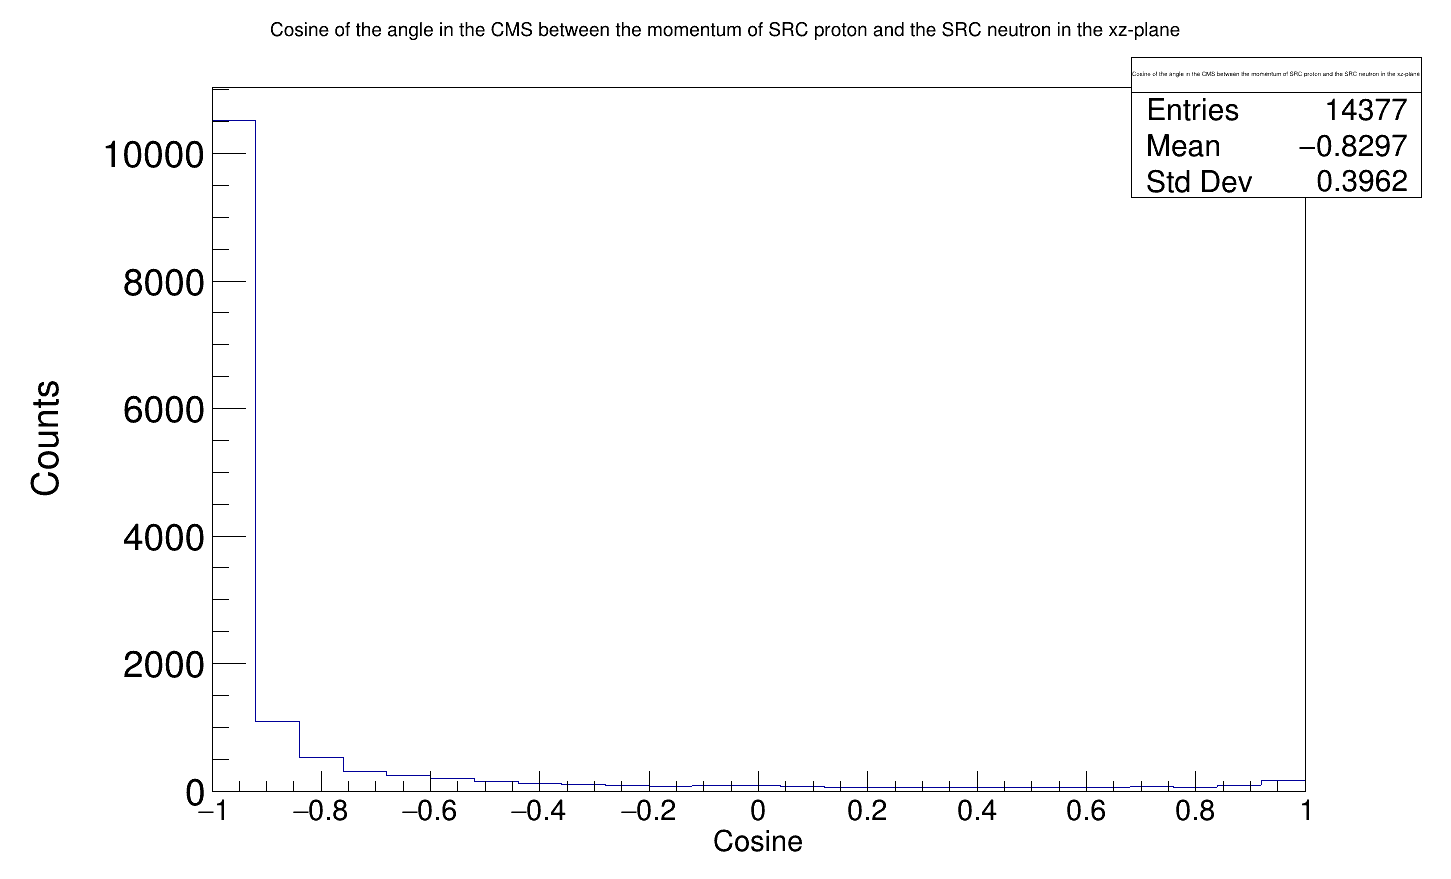
\includegraphics[width=\linewidth]{cos_src_pair.png}
  \caption{Cosine between the recoil nucleon and missing momentum.}
\end{figure}
\newline
\begin{figure}[!htb]
  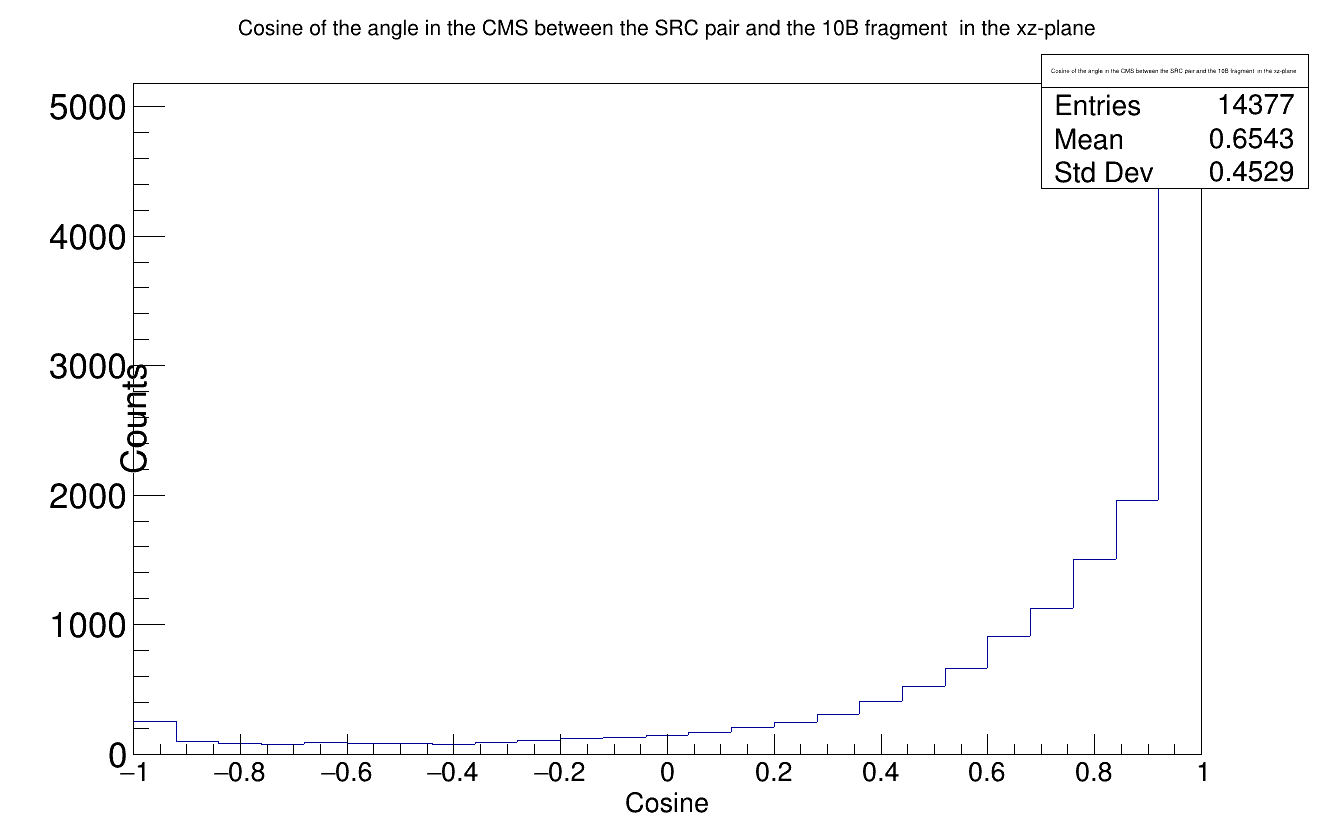
\includegraphics[width=\linewidth]{cos_src_pair_vs_10B.png}
  \caption{Cosine of the angle between the 10B fragment and pair relative momentum.}
  \label{fig:factorization}
\end{figure}
\newline
\newpage

\section{To Dos and Open Questions}
\begin{itemize}
\item plot momentum of 10B fragment versus missing momentum
\item plot mandelstam variables and compare to plots from \url{https://www.nature.com/articles/s41567-021-01193-4}
\item Analyze the plot \ref{fig:factorization} in more detail. This should actually be an uniform flat distribution (slightly shaped according to the acceptance of the detectors). It's not so the case in \ref{fig:factorization}.
\item the angular distribution in \ref{fig:11b_p_i_distr} is not as expected. We would expect back-to-back momenta in the 12C rest frame. When transforming it back to the 11B  rest frame (in z-direction) instead we get the following plot:\newline
\begin{figure}[!htb]
  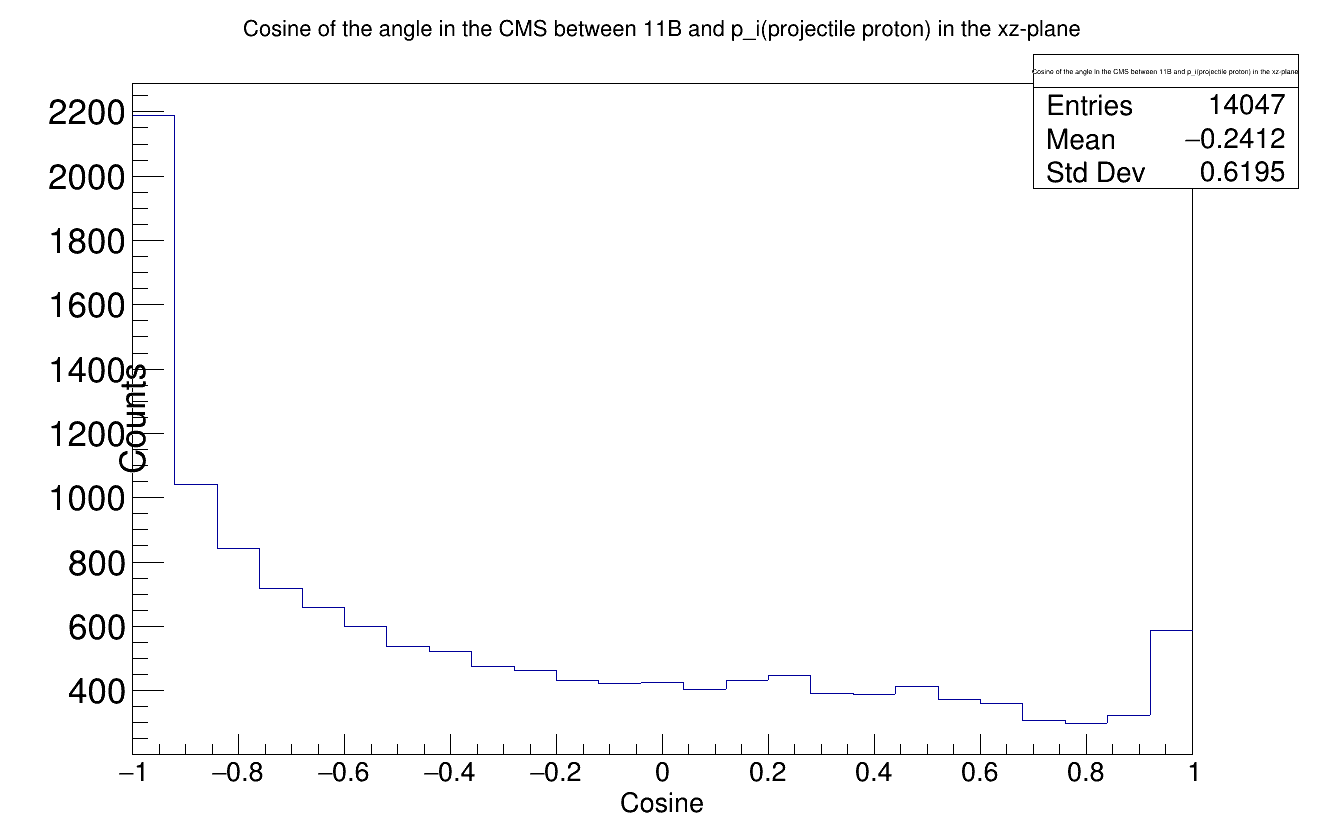
\includegraphics[width=\linewidth]{cos_11b_back_to_back.png}
	\caption{Distribution between the cosine of the opening angle between the missing and fragment momentum in the 11B rest frame (in z-direction)}
\end{figure}
\newline
As beam energy for 12C I use the value 400AMeV. It seems for me that it is set too high and attenuated down the beamline....
\item the 12C(p,2p)10B reaction can come from src,(p,pd) or direct removal of neutron. In \ref{fig:theta1_theta2_distr} we see two small peaks beyond 80 degrees. Could those be a hint for proton-deuteron scattering? Should I use a selection cut as in \url{https://www.nature.com/articles/s41567-021-01193-4} ($p_{miss} \geq 350 MeV$). For the neutron removal, do I have to look into the NEULAND data or should I already see some excited states in the gamma spectrum?
\item plot gamma spectrum for 12C(p,2p)10B.
\item look at high energy runs ($750 MeV$). In this configuration some of the QE scattered protons won't be stopped. What interesting info would I gain when looking at this data? 
\item compare all the above plots with the simulated data that can be retrieved by the QFS generator.
\end{itemize}

\end{document}

